% !TeX root = ../../anexos_logica.tex
\chapter*{Anexo 4-X — Detalle de implantación y catálogos técnicos}
\phantomsection\label{anx:X}
\markboth{Anexo 4-X — Detalle técnico}{Anexo 4-X — Detalle técnico}
\addcontentsline{toc}{chapter}{Anexo 4-X — Detalle de implantación y catálogos técnicos}
Este anexo conserva el detalle de ambientes, emplazamiento, servicios y derivaciones trasladado desde 4.2. El cuerpo mantiene las decisiones, los resultados y las condiciones de aceptación. Los identificadores de componentes y de las Figuras 19--23 se conservan. El traslado no altera la solución ni acredita nuevas pruebas.

\begingroup
\renewcommand{\thesection}{4-X.\arabic{section}}
\renewcommand{\theHsection}{anexo4x.\arabic{section}}
\setcounter{section}{0}
\section{Ciclo de entrega por ambiente}
\label{anx:X-ambientes}
La síntesis y las condiciones obligatorias de promoción permanecen en \href{LAFROX-Subdocumento4.pdf#sub:1-ambientes-de-despliegue-rt-04-01}{4.2.4.1 del cuerpo}. Las figuras siguientes conservan la numeración original; sus pasos se leen junto con los controles del pipeline, la liberación y las ventanas de ese apartado.
\providecommand{\minititulo}[1]{\par\addvspace{8pt}\noindent{\intersemibold\color{lafroxTinta}#1}\par\nopagebreak\addvspace{2pt}}
\setcounter{figure}{18}
\renewcommand{\thefigure}{\arabic{figure}}
\minititulo{Desarrollo}

La Figura~\ref{fig:amb-desarrollo} muestra cómo llega una entrega a Desarrollo. Sus pasos numerados se leen de izquierda a derecha.

\begin{figure}[htbp]\centering
  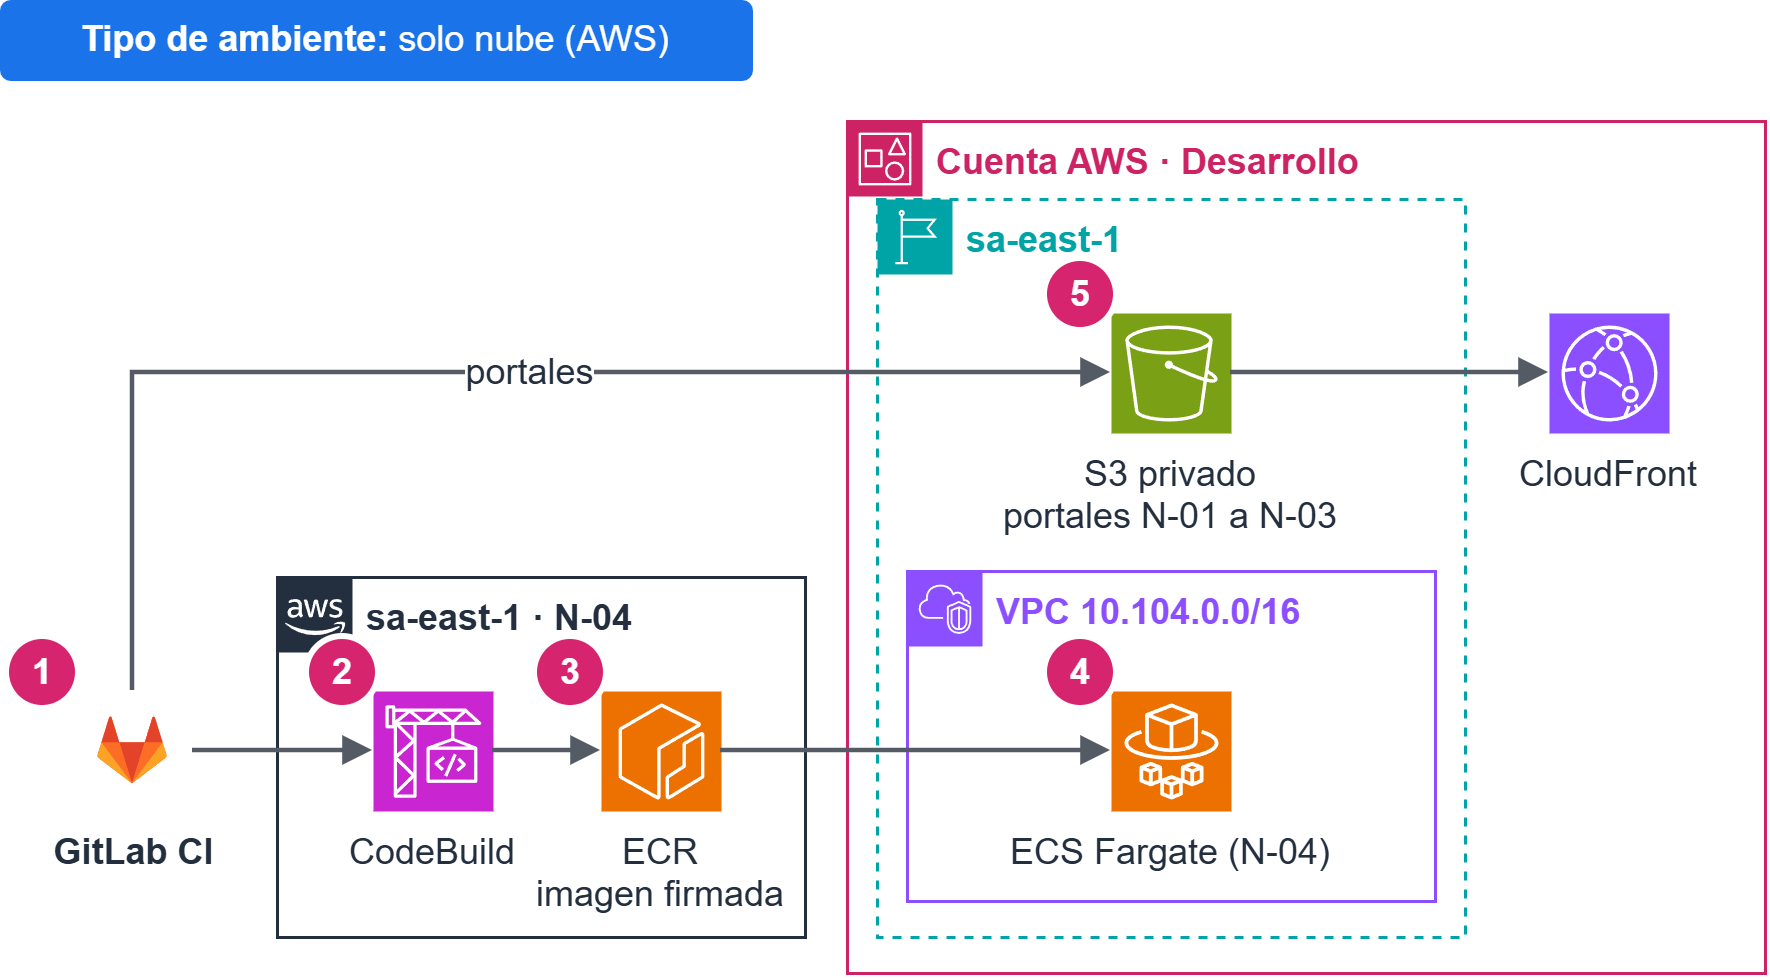
\includegraphics[width=\textwidth]{figuras/fisica/ambientes/amb_desarrollo.png}
  \caption{Ambiente de Desarrollo}\label{fig:amb-desarrollo}
  {\fontsize{9pt}{11pt}\selectfont\raggedright Fuente: (Bases Técnicas Transversales, cap.~4, pp.~10--11), para los ambientes obligatorios, y (Subdocumento 4, diseño de este apartado, \href{LAFROX-Subdocumento4.pdf#fuente-11-j-despliegue}{apartado 4.2.4.1}).\par}
\end{figure}
\FloatBarrier

Los pasos de la figura son los siguientes:

\begin{enumerate}
  \item GitLab CI toma el cambio aprobado en la rama protegida y ejecuta los controles del pipeline, que se detallan más adelante en esta sección.
  \item AWS CodeBuild construye la imagen de la aplicación una sola vez, de forma hermética y con procedencia SLSA nivel 3.
  \item Elastic Container Registry (ECR) guarda la imagen firmada. Desde aquí se promueve por su digest a los demás ambientes, sin recompilar.
  \item ECS Fargate despliega la imagen en la VPC 10.104.0.0/16 de la cuenta de Desarrollo, con la configuración de SSM Parameter Store y los secretos de AWS Secrets Manager propios del ambiente.
  \item El pipeline publica los portales Angular de clientes, transportistas y proveedores (N-01 a N-03) en un bucket S3 privado, que CloudFront sirve.
\end{enumerate}

Desarrollo no tiene enlace con los sitios.

\minititulo{QA}

QA repite la secuencia de Desarrollo en su propia cuenta y su propia VPC (Figura~\ref{fig:amb-qa}). No construye una imagen nueva: usa la misma que recorrió Desarrollo, de modo que una falla detectada aquí corresponde al artefacto y no a una recompilación.

\begin{figure}[htbp]\centering
  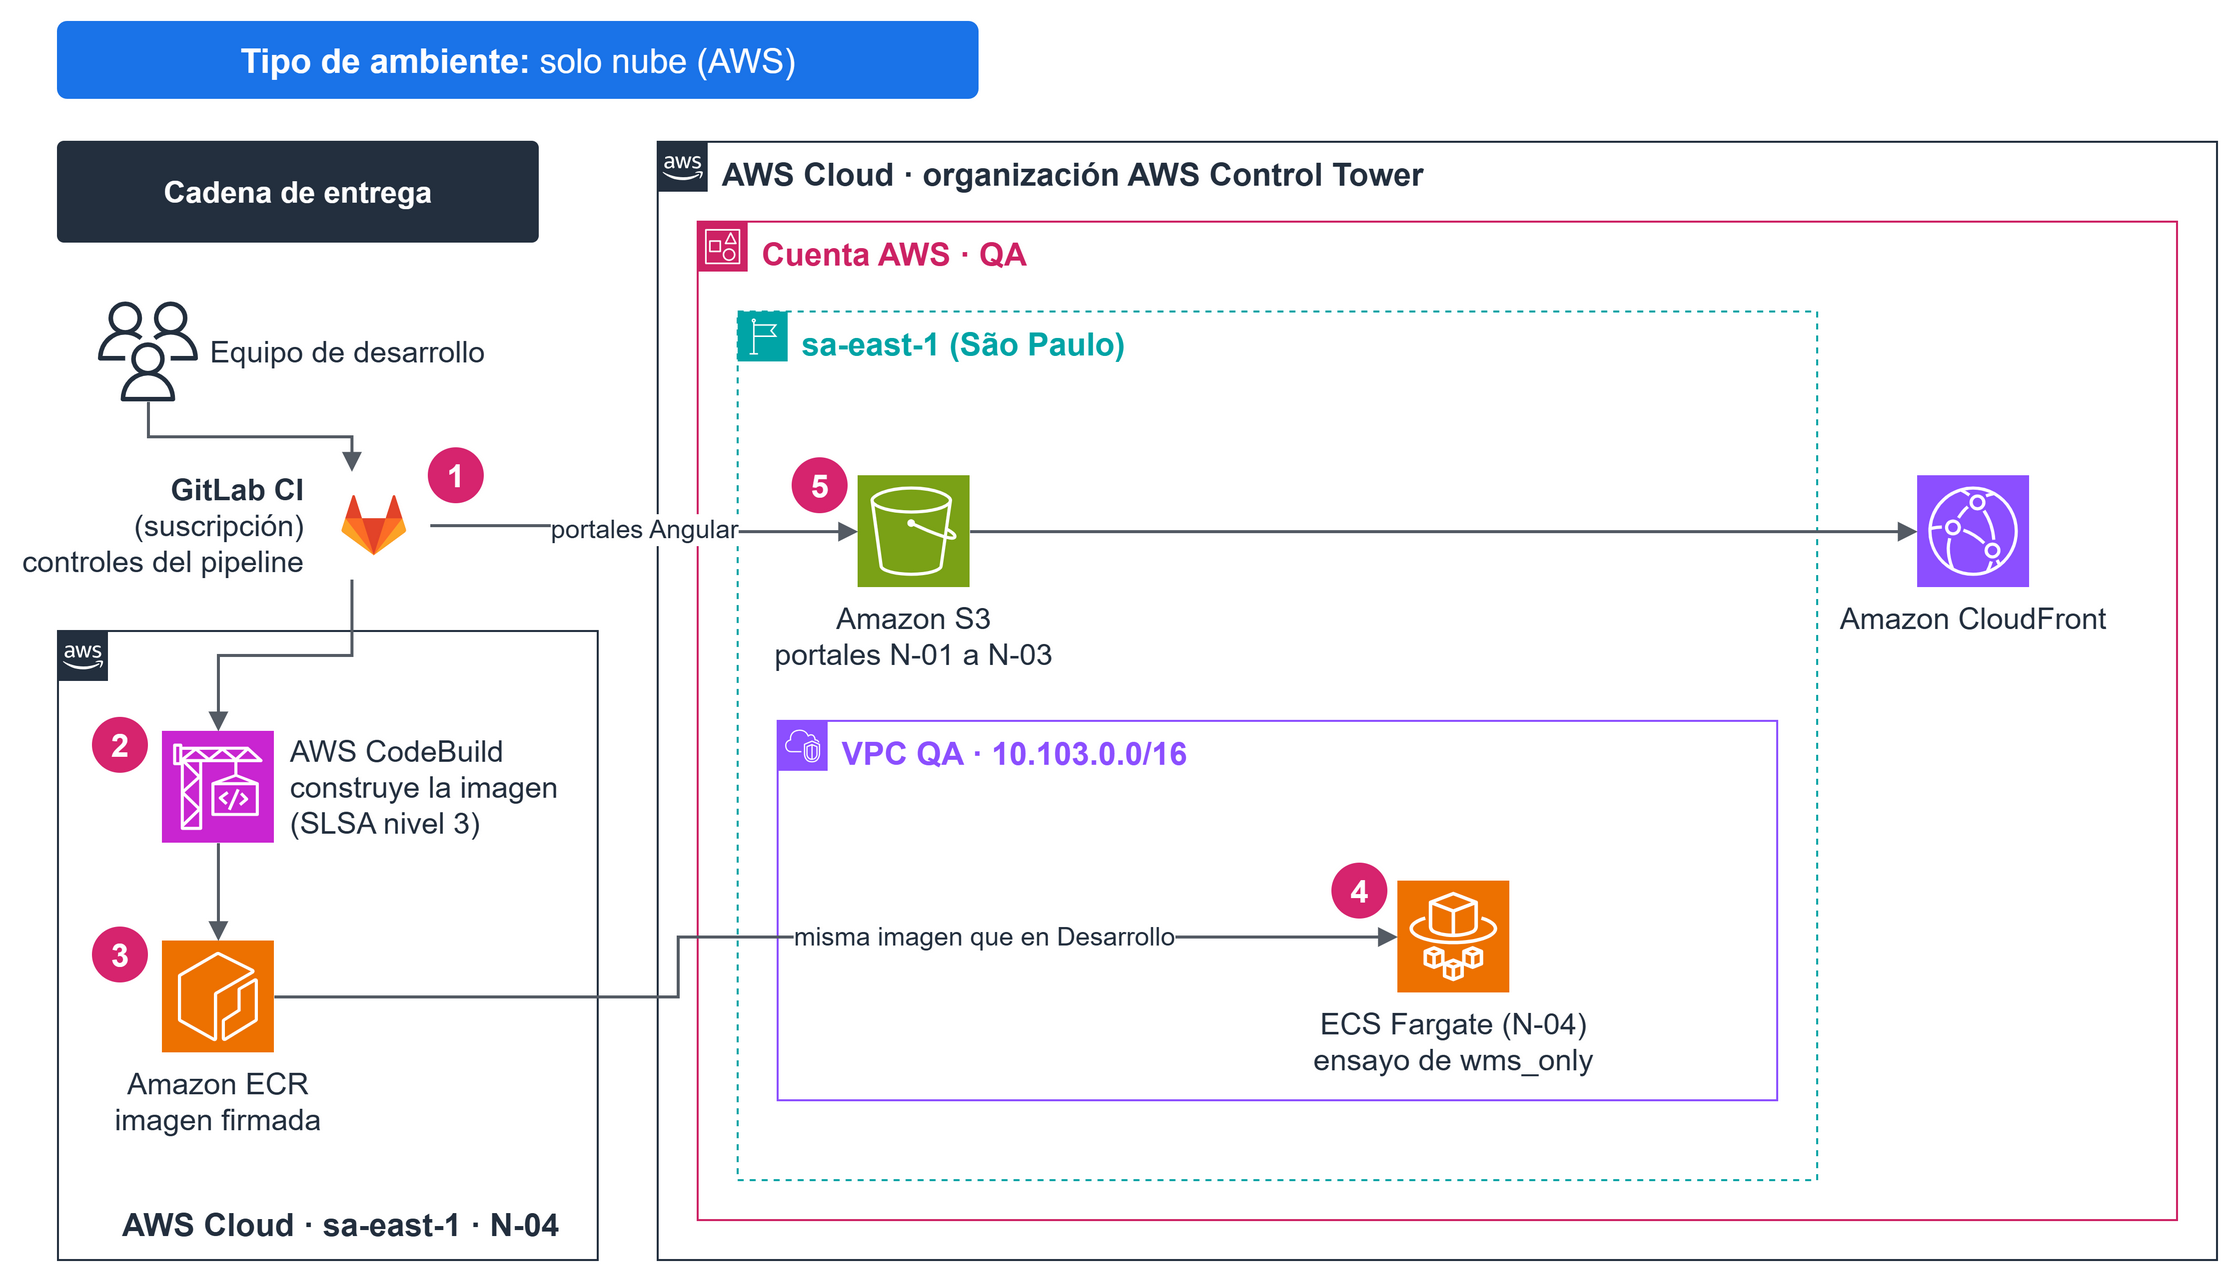
\includegraphics[width=\textwidth]{figuras/fisica/ambientes/amb_qa.png}
  \caption{Ambiente de QA}\label{fig:amb-qa}
  {\fontsize{9pt}{11pt}\selectfont\raggedright Fuente: (Bases Técnicas Transversales, cap.~4, pp.~10--11), para los ambientes obligatorios, y (Subdocumento 4, diseño de este apartado, \href{LAFROX-Subdocumento4.pdf#fuente-11-j-despliegue}{apartado 4.2.4.1}).\par}
\end{figure}
\FloatBarrier

Los pasos de la figura son los siguientes:

\begin{enumerate}
  \item GitLab CI promueve a QA la entrega que superó Desarrollo.
  \item CodeBuild no vuelve a construir: la imagen es la que construyó para Desarrollo.
  \item ECR entrega esa imagen firmada, identificada por su digest.
  \item ECS Fargate la despliega en la VPC 10.103.0.0/16 de la cuenta de QA, donde corren las pruebas funcionales, de integración y de regresión.
  \item Los portales se publican en el bucket S3 privado de QA, que CloudFront sirve.
\end{enumerate}

\minititulo{Preproducción}

En Preproducción la secuencia se ensaya sobre la topología de Producción y sobre un sitio on-premise emulado (Figura~\ref{fig:amb-preproduccion}). Aquí se demuestran las migraciones y el despliegue azul-verde con canario antes de cada paso a producción (RT-04.07, Bases Técnicas Transversales, cap. 4, p. 11).

\begin{figure}[htbp]\centering
  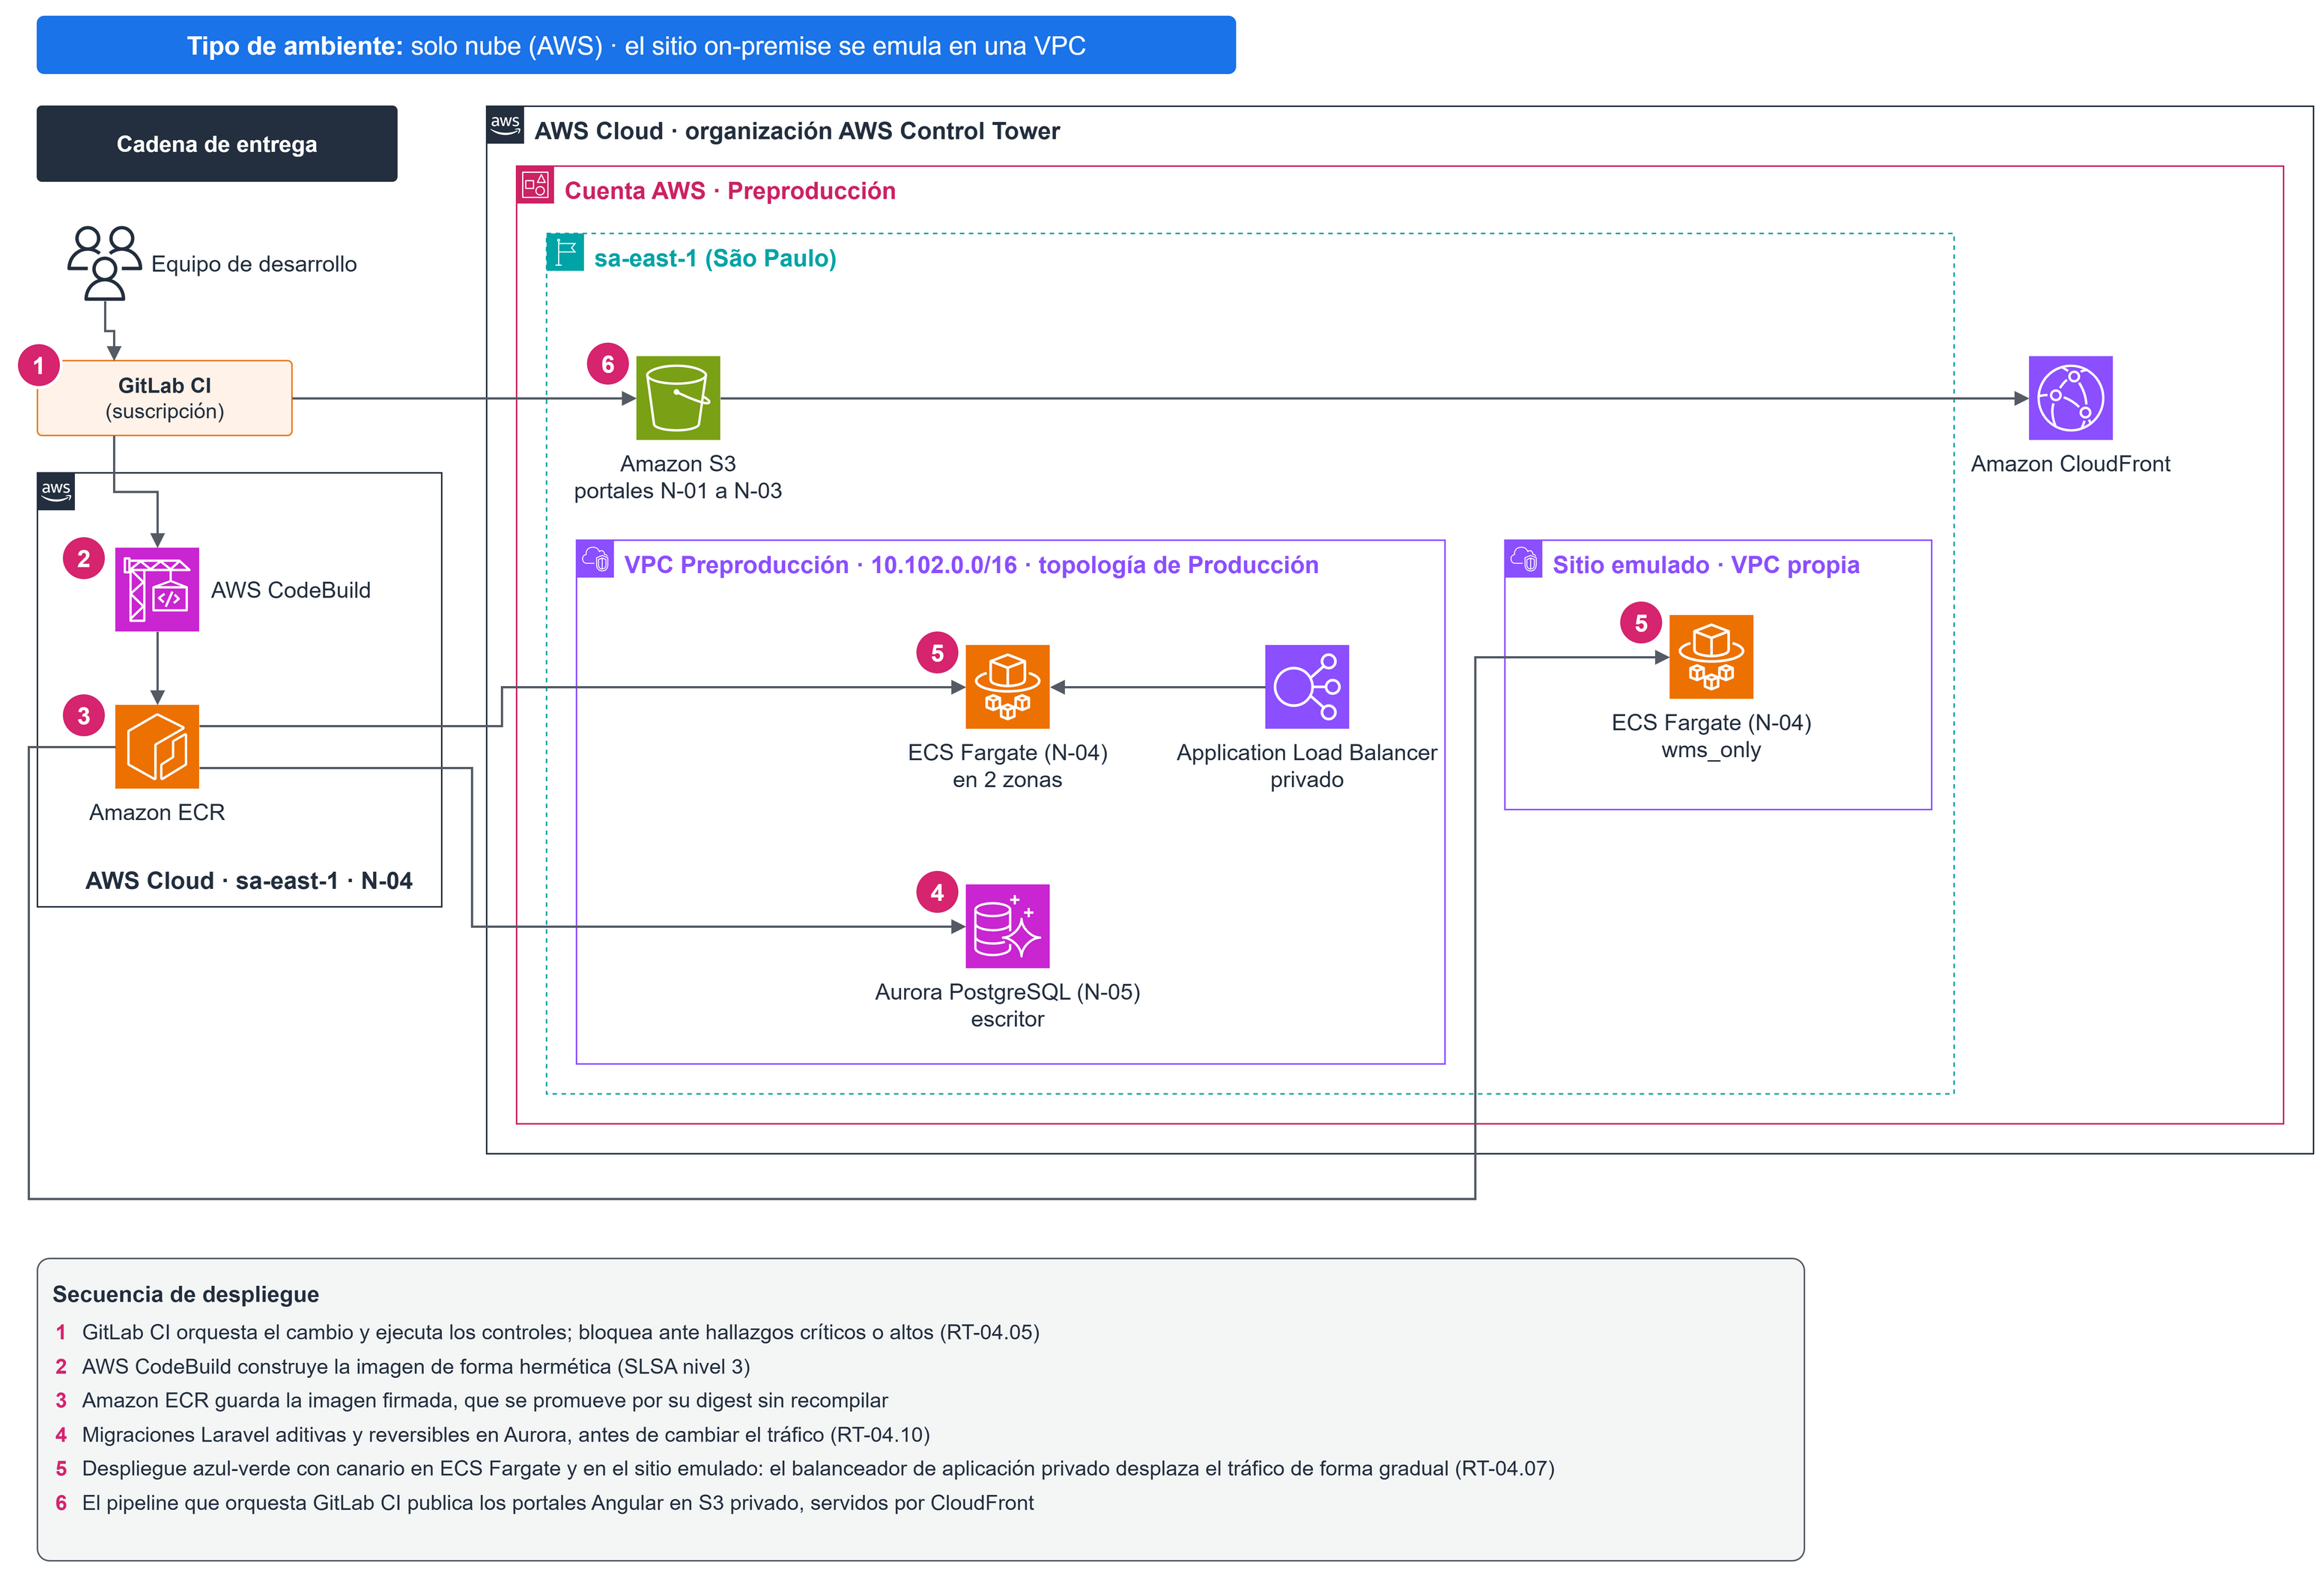
\includegraphics[width=\textwidth]{figuras/fisica/ambientes/amb_preproduccion.png}
  \caption{Ambiente de Preproducción}\label{fig:amb-preproduccion}
  {\fontsize{9pt}{11pt}\selectfont\raggedright Fuente: (Bases Técnicas Transversales, cap.~4, pp.~10--11), para los ambientes obligatorios, y (Subdocumento 4, diseño de este apartado, \href{LAFROX-Subdocumento4.pdf#fuente-11-j-despliegue}{apartado 4.2.4.1}).\par}
\end{figure}
\FloatBarrier

Los pasos de la figura son los siguientes:

\begin{enumerate}
  \item GitLab CI promueve a Preproducción la entrega que superó QA.
  \item CodeBuild no vuelve a construir: la imagen es la misma de Desarrollo y QA.
  \item ECR entrega la imagen firmada por su digest.
  \item Las migraciones aditivas se aplican sobre el escritor de Aurora PostgreSQL (N-05), como un paso único antes de cambiar el tráfico.
  \item La entrega nueva se despliega al mismo tiempo en dos lugares, por lo que la figura asigna el número 5 a ambos:
  \begin{itemize}
    \item En la VPC 10.102.0.0/16 se ensaya el despliegue azul-verde con canario. La entrega vigente («azul») sigue atendiendo mientras ECS Fargate levanta la nueva («verde») a su lado. El balanceador privado, en dos zonas, le pasa primero a la nueva una parte pequeña del tráfico, llamada canario, y la aumenta por etapas mientras no aparezcan errores. Si aparecen, el tráfico vuelve completo a la entrega vigente.
    \item En la VPC del sitio emulado, su base local recibe las mismas migraciones aditivas y la imagen \texttt{wms\_only} recibe la misma entrega mientras el sitio está desconectado. Al reconectarlo, se comprueba que la reconciliación acepta los sobres que dejó la entrega previa.
  \end{itemize}
  \item Los portales se publican en el bucket S3 privado de Preproducción, que CloudFront sirve.
\end{enumerate}

La VPC del sitio emulado no tiene túnel hacia las bodegas, de modo que ningún ensayo alcanza la operación real.

\minititulo{Producción}

En Producción la secuencia se ejecuta de forma automática y llega además a los sitios on-premise (Figura~\ref{fig:amb-produccion}).

\begin{figure}[!htbp]\centering
  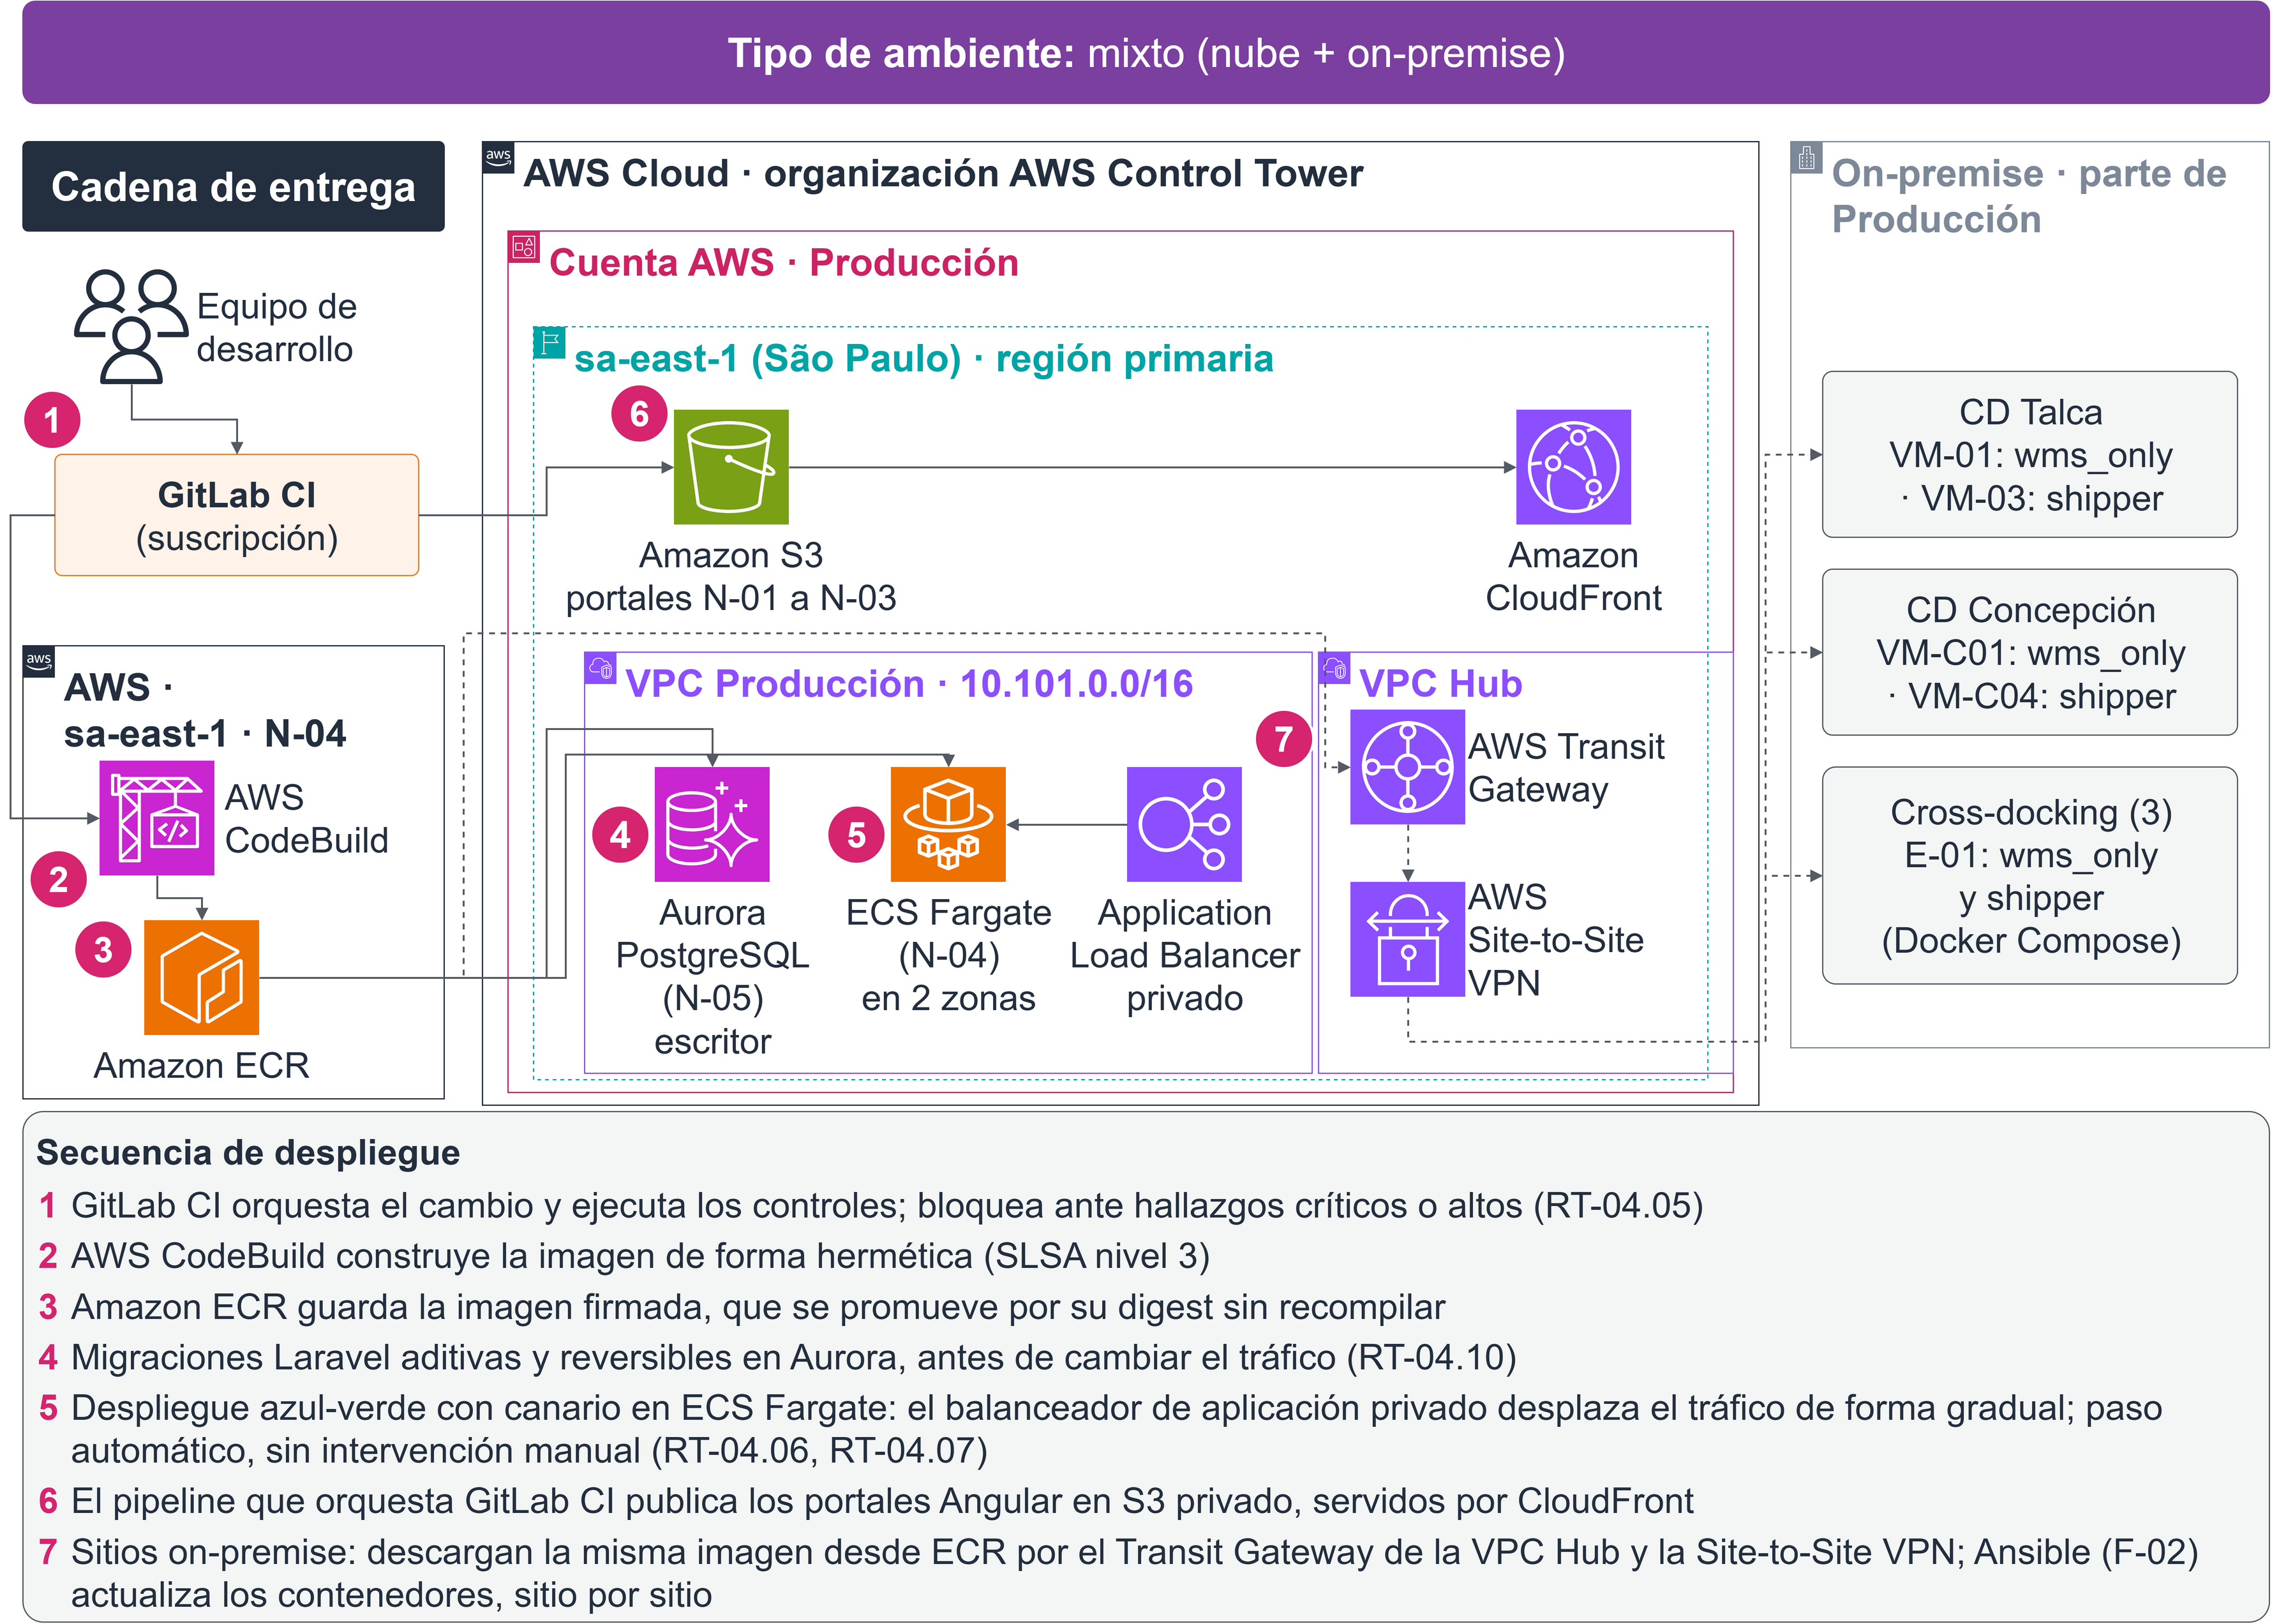
\includegraphics[width=\textwidth]{figuras/fisica/ambientes/amb_produccion.png}
  \caption{Ambiente de Producción}\label{fig:amb-produccion}
  {\fontsize{9pt}{11pt}\selectfont\raggedright Fuente: (Bases Técnicas Transversales, cap.~4, pp.~10--11), para los ambientes obligatorios, y (Subdocumento 4, diseño de este apartado, \href{LAFROX-Subdocumento4.pdf#fuente-11-j-despliegue}{apartado 4.2.4.1}).\par}
\end{figure}

\FloatBarrier

Los pasos de la figura son los siguientes:

\begin{enumerate}
  \item GitLab CI inicia el paso a producción cuando la entrega superó los controles del pipeline y el ensayo en Preproducción, dentro de las ventanas de la Tabla~\href{LAFROX-Subdocumento4.pdf#tab:jd02}{9}.
  \item CodeBuild no vuelve a construir: la imagen es la misma que se ensayó.
  \item ECR entrega la imagen firmada por su digest.
  \item Las migraciones aditivas se aplican sobre el escritor de Aurora PostgreSQL (N-05).
  \item ECS Fargate aplica en la VPC 10.101.0.0/16, en dos zonas, el mismo despliegue azul-verde con canario que se ensayó en Preproducción: la entrega nueva recibe el tráfico por etapas y, si falla, el tráfico vuelve a la vigente.
  \item Los portales se publican en el bucket S3 privado de Producción, que CloudFront sirve.
  \item La entrega llega a los sitios mediante dos acciones que ocurren juntas, por lo que la figura asigna el número 7 a ambas:
  \begin{itemize}
    \item Los sitios descargan la misma imagen desde ECR por la VPN, la VPC Hub y los endpoints de interfaz de la VPC de Producción, en conexiones salientes y sin pasar por Internet.
    \item Ansible (F-02), desde CD Talca, aplica sitio por sitio las migraciones aditivas a la base PostgreSQL activa: VM-02, VM-C02 y la del E-01 activo. En Concepción y los cross-docking, la réplica sincrónica las lleva al equipo en espera. Luego actualiza los contenedores: VM-01, VM-03 y VM-04 en Talca, VM-C01 y VM-C04 en los dos servidores de Concepción y los dos E-01 de cada cross-docking, primero el equipo en espera y luego el activo.
  \end{itemize}
\end{enumerate}

El paso 7 distingue a Producción de los demás ambientes: es el único que llega a las bodegas.

\minititulo{Recuperación ante Desastres}

La Figura~\ref{fig:amb-recuperacion} muestra las dos rutas de recuperación: ante la pérdida de la región primaria y ante la pérdida de la sala de Talca.

\begin{figure}[!ht]\centering
  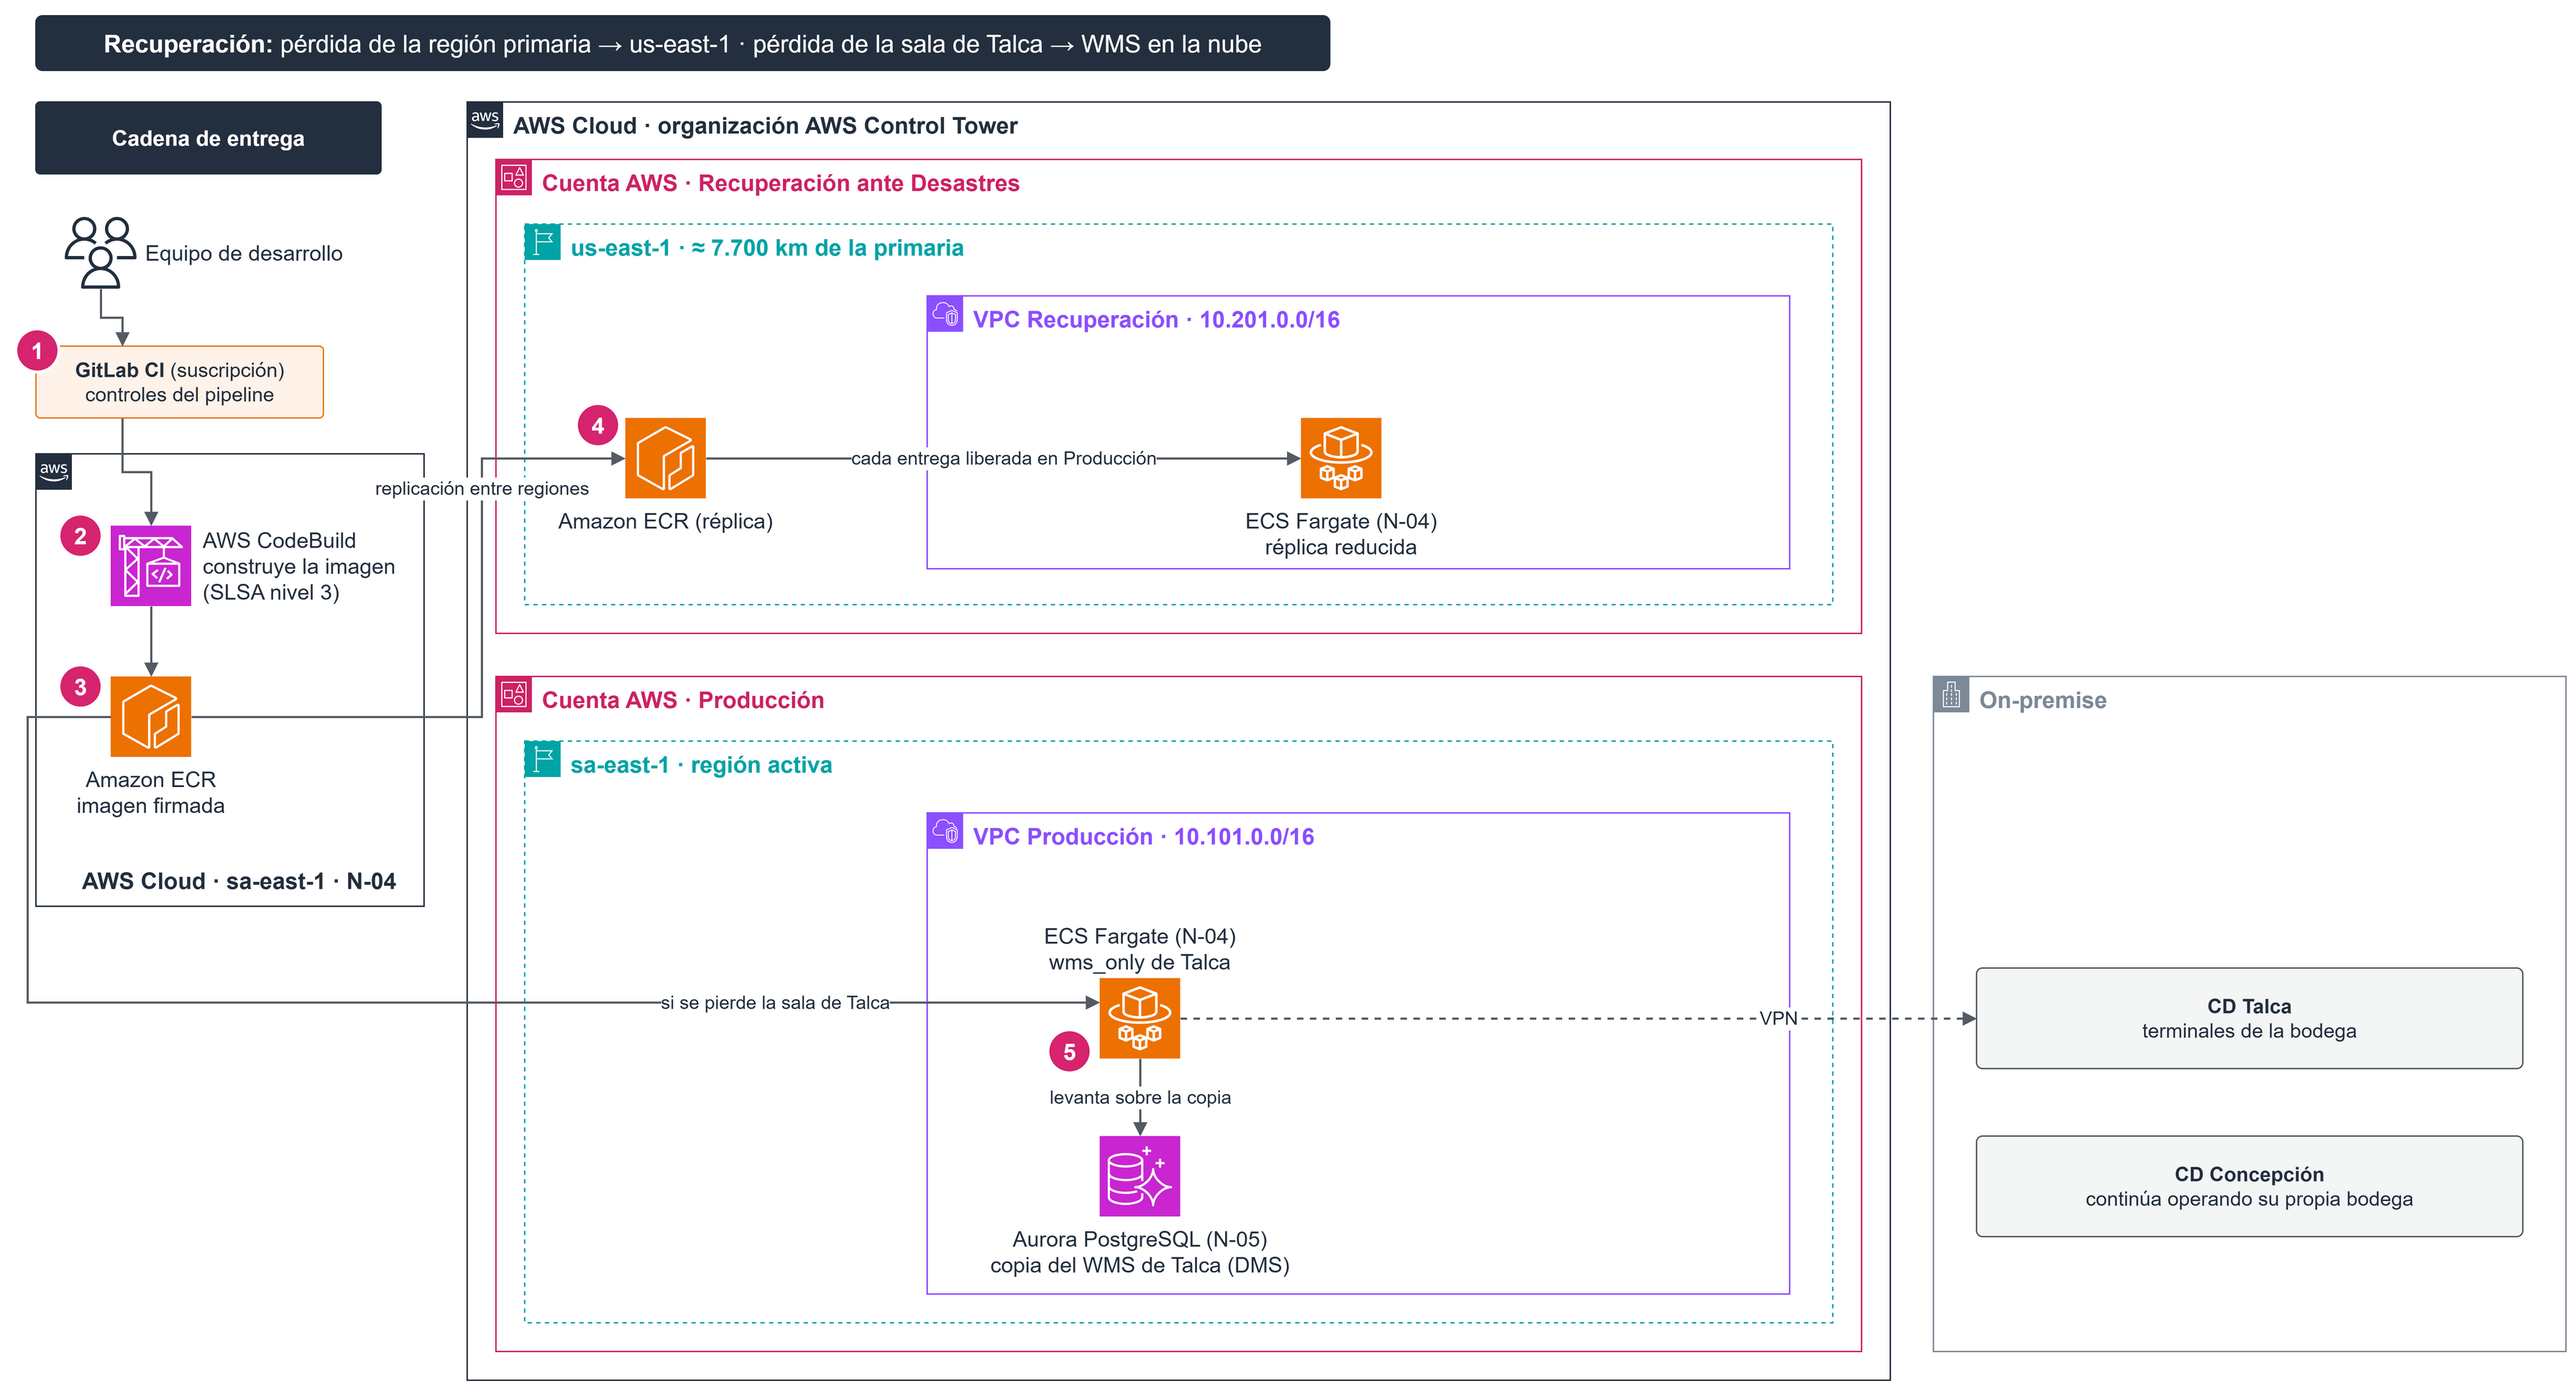
\includegraphics[width=\textwidth]{figuras/fisica/ambientes/amb_recuperacion.png}
  \caption{Ambiente de Recuperación ante Desastres}\label{fig:amb-recuperacion}
  {\fontsize{9pt}{11pt}\selectfont\raggedright Fuente: (Bases Técnicas Transversales, cap.~4, pp.~10--11), para los ambientes obligatorios, y (Subdocumento 4, diseño de este apartado, \href{LAFROX-Subdocumento4.pdf#fuente-11-j-despliegue}{apartado 4.2.4.1}).\par}
\end{figure}

Los pasos de la figura son los siguientes:

\begin{enumerate}
  \item GitLab CI libera la entrega en Producción.
  \item CodeBuild no vuelve a construir: la imagen es la misma que se liberó en Producción.
  \item ECR guarda la imagen firmada en sa-east-1.
  \item ECR replica cada entrega liberada en Producción a us-east-1, y la réplica reducida de ECS Fargate la despliega en la VPC 10.201.0.0/16. Si se pierde la región primaria, esa réplica escala a carga completa en menos de 30 minutos.
  \item Si se pierde la sala de Talca, el perfil \texttt{wms\_only} de Talca se levanta en ECS Fargate de la VPC de Producción, sobre la copia del WMS de Talca que AWS DMS mantiene en Aurora PostgreSQL (N-05). El WMS recuperado conserva la identidad de Talca y atiende a los terminales de la bodega por la VPN.
\end{enumerate}

Concepción no depende de esta recuperación: sigue operando su propia bodega.

Las cinco figuras comparten la misma cadena de entrega y la misma imagen firmada, y difieren en la cuenta, el bloque de direccionamiento y el alcance hacia los sitios. Solo Producción llega a las bodegas por la VPC Hub, y Recuperación ante Desastres conserva preparada la réplica reducida de us-east-1 y la recuperación del WMS de Talca en la nube.
\FloatBarrier
\section{Catálogo razonado de emplazamiento}
\label{anx:X-emplazamiento}
Se conservan los 36 componentes: trece de nube, once locales y doce híbridos. La síntesis por criterio y las condiciones de autonomía permanecen en \href{LAFROX-Subdocumento4.pdf#fuente-02-a-emplazamiento}{4.2.2 del cuerpo}; T-11 mantiene cantidades y especificaciones.

\subsection*{Componentes de nube pura}
\phantomsection\label{anx:X-nube}
\begin{itemize}
  \item \textbf{N-01 Portal de Clientes} (regulación): atiende el catálogo, el pedido de autoatención, el estado de entrega, los documentos y el saldo de los clientes desde Internet, también como aplicación instalable que arma el pedido sin señal. Por eso se publica solo en la DMZ de la nube y ningún tráfico externo llega a los sitios del CLIENTE.
  \item \textbf{N-02 Portal de Transportistas} (regulación): desde la Etapa 2, los representantes de cada empresa transportista consultan rutas y documentos y confirman conductor y vehículo desde Internet, y ese acceso se resuelve en la DMZ de la nube. Los conductores externos no usan el portal: trabajan en la app de reparto con su identidad personal.
  \item \textbf{N-03 Portal de Proveedores} (regulación): los 180 proveedores consultan órdenes de compra, recepciones y devoluciones desde Internet, aislados de la red de bodega.
  \item \textbf{N-04 Plataforma de aplicación} (costo): Laravel corre en ECS Fargate con perfiles de API, reconciliación, trabajos y planificación que escalan por separado. La plataforma aloja el frontend Angular de consolas y el transporte AS2 de M11 en dos tareas distribuidas entre dos zonas cada uno. El motor de rutas M4 ejecuta una tarea por corrida, que ECS relanza en otra zona ante una falla para repetirla dentro de la planificación de 15:00 a 18:30, con el plazo de 20 min por corrida medido en la prueba de aceptación. M11 usa contratos versionados (ADR-11, Anexo 4-O).
  \item \textbf{N-05 Base de datos en nube} (criticidad): Aurora PostgreSQL guarda el transaccional de los módulos en nube y la réplica del WMS, conmuta entre zonas en menos de 30 s y se replica a us-east-1.
  \item \textbf{N-06 Telemetría cruda} (volumen): DynamoDB recibe las lecturas de temperatura sin gestión de capacidad y las expira a los 30 días, cuando ya están consolidadas en la capa analítica.
  \item \textbf{N-07 Caché} (latencia): ElastiCache mantiene en memoria el stock, el crédito y las sesiones para que la consulta de preventa responda en menos de 2 s.
  \item \textbf{N-08 Ingesta de IoT} (volumen): recibe 30.548 mensajes diarios por IoT Core y CloudConnect/SQS, asociados a 127.848 lecturas. M9 persiste evento y obligación de aviso juntos en Aurora, confirma A2 y actualiza DynamoDB. Móvil y satélite se concilian por productor, arranque y secuencia.
  \item \textbf{N-09 Mensajería} (criticidad): una cola SQS FIFO recibe la reconciliación de los sitios como sobres JSON versionados, en orden por grupo y sin duplicados. Otra cola FIFO lleva las solicitudes al ERP hasta \texttt{erp-sync} y una cola FIFO de respuesta para Concepción y para cada cross-docking devuelve sus respuestas, porque Talca las recibe por RabbitMQ local. Una cola FIFO de coordinación por cada uno de los cinco sitios lleva las solicitudes de retención y liberación de stock que su shipper lee por conexión saliente. Otras colas SQS, separadas de esas, transportan los trabajos internos de Laravel, y SNS difunde las alertas de excursión térmica.
  \item \textbf{N-10 Plataforma analítica} (volumen y costo): S3, Glue, Redshift Serverless y QuickSight conservan 5 años de datos separados del transaccional. Los tableros y la autoría de QuickSight se integran en las consolas para usuarios registrados, con modelo semántico documentado, creación autónoma de informes, exportación y permisos separados de lectura y creación. Los indicadores operacionales actuales se consultan en la API de negocio.
  \item \textbf{N-11 Respaldo inmutable y réplica} (regulación): S3 Object Lock, AWS Backup y la réplica en us-east-1 guardan la copia que ni un administrador puede borrar y sostienen el RTO de 4 h y el RPO de 15 min.
  \item \textbf{N-12 Seguridad y gobierno} (regulación): KMS, Secrets Manager, WAF, Shield Advanced, Verified Access, Security Lake y CloudWatch implementan en la nube los controles del Artículo 21 de las Bases Administrativas (art. 21, p. 15) definidos en la arquitectura de seguridad (apartado 4.1), como servicios que un equipo de TI de cuatro personas puede operar.
  \item \textbf{N-13 Gestión de dispositivos} (costo): Microsoft Intune, con inscripción Android Enterprise y las herramientas Zebra DNA, gestiona como servicio el parque de terminales de preventa, reparto y cámara, con borrado remoto selectivo y sin infraestructura en los sitios.
\end{itemize}

\subsection*{Componentes on-premise}
\phantomsection\label{anx:X-local}
\begin{itemize}
  \item \textbf{B-01 Sensores de temperatura} (latencia): los 21 puntos de medición de las cámaras se leen por Modbus en el mismo sitio, porque dentro de la cámara no hay señal y la lectura no puede esperar al enlace.
  \item \textbf{B-02 Gateway IoT} (latencia): los gateways de Talca y Concepción detectan la excursión crítica y sostenida y bloquean el despacho en menos de 5 s, con un buffer de 24 h si cae el enlace, igual a la autonomía del centro de distribución.
  \item \textbf{C-03 Terminales de bodega} (conectividad): los terminales MC9400 trabajan en la bodega y en las cámaras, incluido el congelado a $-$22\,\textdegree{}C, sin señal móvil, contra el WMS del sitio por la red inalámbrica de la bodega.
  \item \textbf{C-04 Impresoras de andén} (latencia): las seis impresoras ZT411 imprimen la etiqueta SSCC en el andén al armar la unidad logística, sin salir de la red local.
  \item \textbf{C-05 Balanzas de recepción} (latencia): las tres balanzas envían el peso de recepción al WMS del sitio en línea, sin digitación y sin depender del enlace.
  \item \textbf{D-02 Switching} (criticidad): los switches de cada sitio segmentan la red local por VLAN y la mantienen operativa aunque caiga la WAN.
  \item \textbf{D-03 Enlace de fibra} (conectividad): contratado con Telsur (Grupo Gtd), es el camino principal de la VPN en Talca y Concepción, con 20 y 10 Mbps en régimen.
  \item \textbf{D-04 Enlace LTE} (conectividad): respalda la fibra en los CD con Entel, operador distinto de Telsur, y, con Entel y Claro, respalda a Starlink en los cross-docking, con conmutación en menos de 30 s.
  \item \textbf{D-06 Enlace satelital} (conectividad): Starlink es el camino principal de los cross-docking, respaldado por LTE de Entel y Claro, y el tercer camino en espera caliente de Talca y Concepción, con terminal encendido, túnel IPsec establecido y BGP de menor preferencia que solo toma tráfico si fallan fibra y LTE.
  \item \textbf{E-01 WMS de cross-docking} (criticidad): el par de mini-PC de cada plataforma, uno activo y otro en espera, opera 100\,\% en local la ventana de 3 h de recepción, desconsolidación y re-despacho, con su propio broker y su propia base, replicada al equipo en espera.
  \item \textbf{F-02 Gestión de parches} (costo): Ansible aplica los parches y las líneas base CIS a los nodos de los cinco sitios por la red de gestión, sin licencia de plataforma.
\end{itemize}

\subsection*{Componentes híbridos}
\phantomsection\label{anx:X-hibridos}
\begin{itemize}
  \item \textbf{A-01 Motor WMS} (latencia): el perfil \texttt{wms\_only} del artefacto Laravel, con su servidor web y PHP-FPM, corre en VM-01, VM-C01 y E-01 porque la confirmación de preparación debe responder en 1 s sin depender del enlace, y su réplica en Aurora sostiene la continuidad. El mismo motor expone la puerta de API local de la bodega, que durante un corte valida el esquema, la tasa, el UUID y la auditoría de las solicitudes de los terminales sin pasar por API Gateway.
  \item \textbf{A-02 Base transaccional del WMS} (criticidad): PostgreSQL 16 en VM-02 y VM-C02 es el registro de cada bodega durante un corte. AWS DMS replica continuamente los cambios de VM-02 (Talca) a Aurora para continuidad y lectura por fibra, LTE o Starlink. VM-C02 (Concepción) entrega sus eventos por las colas de integración. En Concepción y en cada cross-docking, la base activa se replica en forma sincrónica al equipo en espera.
  \item \textbf{A-03 Broker de colas} (conectividad): RabbitMQ en VM-03, VM-C04 y E-01 guarda hasta 24 h de eventos sin enlace, con mensajes persistentes y confirmación de publicación. El shipper, un proceso PHP con el adaptador AMQP \texttt{php-amqplib}, los publica como sobres JSON en SQS FIFO y solo los retira del broker cuando SQS confirma la recepción. El outbox conserva 24 h de eventos ya enviados para reenviarlos tras una conmutación.
  \item \textbf{A-04 Capa anticorrupción del ERP} (criticidad): corre en VM-04, en la misma sala que el ERP de 2017, que no se modifica. En la misma VM, \texttt{erp-sync} consume la cola local de Talca y, mediante conexión saliente, la cola FIFO de solicitudes al ERP de los demás orígenes, cuyas respuestas devuelve por la cola de cada sitio. Usa una clave idempotente por operación para que un reintento no emita un segundo documento tributario.
  \item \textbf{A-05 Identidad} (conectividad): el IdP maestro Keycloak corre en Fargate y sus cachés de solo lectura en VM-05, VM-C03 y E-01 validan las sesiones de bodega y de cross-docking sin enlace. En el mismo nodo, un verificador local habilita cada relevo de turno durante un corte con el manifiesto de turno firmado y un segundo factor local, el PIN personal.
  \item \textbf{B-03 a B-15 Kit de camión} (conectividad): los 28 camiones (18 propios y 10 de transportistas) llevan gateway Greengrass, tres PT100 e ioLogik, simuladores, sensor independiente, termógrafo EN 12830 cada 1 min e Iridium Edge. Estos equipos los adquiere el CLIENTE según la especificación del Formulario T-11, y LafroX los instala y mantiene; las SIM M2M B-15 se contratan como servicio. El gateway detecta y alarma por cable; el TC58e recibe latido por Wi-Fi local y lee los registradores por Bluetooth. Móvil e Iridium transmiten siempre en paralelo; la protección local no depende de ninguno. Al regreso se descargan y concilian las tres series antes de sellar el expediente.
  \item \textbf{C-01 App de preventa} (conectividad): toma pedidos contra el almacén local del terminal cuando no hay señal y sincroniza por CloudFront al reconectar, sin duplicar pedidos (sección~\href{LAFROX-Subdocumento4.pdf#fuente-02-c-conexiones}{4.2.5}).
  \item \textbf{C-02 App de reparto} (conectividad): registra entregas, evidencia y cobros durante 14 h sin señal y los sincroniza con la nube al recuperar cobertura.
  \item \textbf{D-01 Firewall y Customer Gateway} (criticidad): el par de firewalls de cada uno de los cinco sitios termina los túneles IPsec hacia el Transit Gateway de AWS y conmutan de enlace en menos de 30 s.
  \item \textbf{D-05 Respaldo local} (conectividad): el NAS WORM de Talca restaura el WMS en 4 h sin depender del enlace, y su complemento inmutable vive en S3 Object Lock.
  \item \textbf{F-01 Telemetría de observabilidad} (conectividad): los colectores ADOT de VM-06, VM-C04 y E-01 guardan hasta 24 h de métricas y trazas en disco y las envían a CloudWatch al reconectar.
  \item \textbf{F-03 Detección en endpoints} (regulación): los agentes EDR de cada nodo y estación reportan a una consola central, lo que da una sola respuesta ante incidentes en nube y on-premise. El servidor del ERP es un activo del CLIENTE que no forma parte de la solución: LafroX lo traslada sin cambiar su software, y el firewall de Talca restringe las entradas al tráfico de la ACL en VM-04 y a la administración autorizada del CLIENTE. Permite las salidas tributarias del ERP hacia el SII por los caminos habilitados, con destinos, puertos y reglas documentados en el levantamiento de INT-07. Esto no habilita escrituras directas de los módulos al ERP.
\end{itemize}

\section{Servicios contratados por función}
\label{anx:X-servicios}
La selección, residencia, contratación y topología permanecen en \href{LAFROX-Subdocumento4.pdf#fuente-02-b-servicios-nube}{4.2.3 del cuerpo}. La relación detallada es:
\begin{itemize}
\item \textbf{Entrada pública.} \textbf{Servicios contratados:} Route 53, CloudFront, AWS WAF, Shield Advanced, API Gateway pública. \textbf{Componentes:} N-01 a N-03, N-12, \textbf{Región:} Global y sa-east-1.
\item \textbf{Acceso interno.} \textbf{Servicios contratados:} Verified Access, API Gateway privada y endpoint execute-api. \textbf{Componentes:} N-04, N-12, \textbf{Región:} sa-east-1 y us-east-1.
\item \textbf{Cómputo de aplicación.} \textbf{Servicios contratados:} ECS Fargate, Application Load Balancer privado, Lambda autorizadora. \textbf{Componentes:} N-04, A-05, \textbf{Región:} sa-east-1 y us-east-1.
\item \textbf{Datos operacionales.} \textbf{Servicios contratados:} Aurora PostgreSQL, Database Migration Service, DynamoDB, ElastiCache. \textbf{Componentes:} N-05, A-02, N-06, N-07, \textbf{Región:} sa-east-1 y us-east-1 para las réplicas declaradas. ElastiCache se reconstruye durante la recuperación.
\item \textbf{Mensajería.} \textbf{Servicios contratados:} SQS FIFO para la reconciliación, para las solicitudes al ERP y sus respuestas, y para la coordinación de reservas por sitio, SQS para los trabajos de Laravel y SNS, con equivalentes vacíos creados por infraestructura como código en us-east-1. \textbf{Componentes:} N-09, A-03, \textbf{Región:} sa-east-1 y us-east-1.
\item \textbf{Notificaciones.} \textbf{Servicios contratados:} Amazon SES, Amazon SNS para SMS y AWS End User Messaging Social. \textbf{Componentes:} N-04 (INT-11). \textbf{Región:} sa-east-1.
\item \textbf{Integración B2B.} \textbf{Servicios contratados:} CloudFront con AWS WAF y Shield Advanced, Application Load Balancer interno y OpenAS2 en Fargate, \textbf{Componentes:} N-04 (M11), \textbf{Región:} sa-east-1.
\item \textbf{Internet de las cosas.} \textbf{Servicios:} IoT Core, Greengrass V2, Iridium CloudConnect y colas SQS de subida, bajada, confirmación y error. \textbf{Componentes:} N-08, B-02, B-03 y gateway del camión. \textbf{Región:} sa-east-1 y borde, segundo destino en us-east-1. CloudConnect se contrata con Globalsat Chile en el paquete 8.2.7 del T-14. Si ese servicio no está disponible, la ingesta usa SBD directo hacia un receptor en ECS, con el mismo contrato de ingesta.
\item \textbf{Analítica.} \textbf{Servicios contratados:} S3, Glue, Redshift Serverless, QuickSight embebido, \textbf{Componentes:} N-10, \textbf{Región:} sa-east-1.
\item \textbf{Respaldo y recuperación.} \textbf{Servicios contratados:} AWS Backup, S3 Object Lock, replicación de S3 entre regiones. \textbf{Componentes:} N-11, D-05, \textbf{Región:} sa-east-1 y us-east-1.
\item \textbf{Red y conectividad.} \textbf{Servicios contratados:} VPC, Transit Gateway, Site-to-Site VPN, NAT Gateway, VPC Endpoints, \textbf{Componentes:} D-01, \textbf{Región:} sa-east-1 y us-east-1.
\item \textbf{Identidad, claves y secretos.} \textbf{Servicios contratados:} KMS, Secrets Manager, Parameter Store, IAM Identity Center, AWS Certificate Manager, AWS Private CA para los certificados privados de mTLS y de la red inalámbrica. \textbf{Componentes:} A-05, N-12, \textbf{Región:} sa-east-1 y us-east-1.
\item \textbf{Detección y cumplimiento.} \textbf{Servicios contratados:} GuardDuty Runtime Monitoring para tareas ECS Fargate, Security Lake, Security Hub, Inspector, Macie, CloudTrail y Config. \textbf{Componentes:} N-12, F-03, \textbf{Región:} sa-east-1 y us-east-1.
\item \textbf{Operación y gobierno.} \textbf{Servicios contratados:} CloudWatch, Systems Manager, AWS Fault Injection Service, Control Tower, Organizations, Cost Explorer, Budgets. \textbf{Componentes:} F-01, F-02, N-12, \textbf{Región:} sa-east-1.
\item \textbf{Construcción y registro de imágenes.} \textbf{Servicios contratados:} CodeBuild y Elastic Container Registry con replicación de imágenes entre regiones, \textbf{Componentes:} N-04, A-01, \textbf{Región:} sa-east-1 y us-east-1.
\item \textbf{Servicios de terceros en nube.} \textbf{Servicios contratados:} Microsoft Intune con Android Enterprise y Zebra DNA, consola del EDR, \textbf{Componentes:} N-13, F-03, \textbf{Región:} Servicio gestionado.
\end{itemize}
\section{Derivaciones complementarias de capacidad}
\label{anx:X-calculos}
Los resultados y criterios de aceptación permanecen en \href{LAFROX-Subdocumento4.pdf#fuente-12-k-dimensionamiento}{4.2.6 del cuerpo}. La memoria completa se entrega en el Anexo 4-W. Se conservan aquí las explicaciones trasladadas del cuerpo para no perder sus supuestos y distinciones.

\subsection*{Derivación por lugar}
El Anexo 4-W.2 deriva el perfil por lugar. SV-03 reparte preparación y despacho entre Talca y Concepción en proporción 2/3 y 1/3. Las plataformas registran tres operaciones de llegada y una de despacho sobre su volumen agregado. La nube reúne preventa, reparto, recepción, trazabilidad, guías, sincronización y EDI. El portal aplica 2.600 ÷ 9 × 2 por SV-04 × 60 ÷ 3.600.

\subsection*{Cotas de guías y sesiones}
El despacho se reparte entre ambos centros conforme a SV-03, en la misma proporción que la preparación. Los aproximadamente 2.852 documentos/día de septiembre son el total de DTE (34.000 ÷ 22,14 × 1,857), no sólo guías. Considerarlos todos como guías que deben emitirse antes de la salida es una cota conservadora. Las 2.600 sesiones diarias del portal son un parámetro de diseño: una por cada cliente de food service y de cadenas, 2.100 + 500 (Bases Técnicas del caso, cap. 2, p. 4), y no son las 2.600 visitas diarias de preventa (Bases Técnicas del caso, anexo B, p. 38). Los objetivos de prueba de septiembre y de despacho se distinguen en la Tabla~\href{LAFROX-Subdocumento4.pdf#tab:t86}{23}.

\subsection*{EDI y pagos}
El EDI actual es cero. Desde enero de 2029 opera todos los días, y se dimensiona con la misma hipótesis en régimen y en peak: 11\,\% de los pedidos, que corresponde a la cadena principal y su 11\,\% de la venta (SV-05), con cuatro mensajes por pedido. Son 1.400 × 11\,\% × 4 = 616 mensajes en régimen y 2.600 × 11\,\% × 4 = 1.144 en peak. La pasarela de pago se acota con un pago electrónico por entrega como máximo y dos mensajes por pago, solicitud y respuesta: 2.800 en régimen y 5.200 en peak. Los 11.800 cobros mensuales del caso son en efectivo y no miden pagos con tarjeta. La Tabla~\href{LAFROX-Subdocumento4.pdf#tab:t81}{18} compara el peor caso del camino principal y el drenaje de los caminos de respaldo.

\subsection*{Capacidad útil y utilización local}
Ceph entrega 1,92 TB útiles con seis NVMe de 960 GB, tres réplicas y sin RAID. Con un nodo caído, Talca conserva 64 vCPU y 128 GB RAM, y Ceph sigue sirviendo los datos con dos réplicas hasta que el nodo vuelve. El umbral de llenado al 80\,\% es 1,54 TB, superior a los 221 GB requeridos a 3×. Su utilización actual es 40,62\,\% de CPU, 46,09\,\% de RAM y 10,94\,\% de disco. A 3× es 40,62\,\%, 47,66\,\% y 11,51\,\%, respectivamente. Cada servidor de Concepción dispone de 16 hilos, 32 GB RAM y 3,84 TB útiles en RAID 10 y aloja el conjunto completo, activo o en espera. Utiliza 75,00\,\% de CPU, 53,12\,\% de RAM y 3,65\,\% de disco actualmente, y 75,00\,\%, 56,25\,\% y 3,65\,\% a 3×. En Talca la redundancia es N+1 dentro del clúster, y sus nodos ofertados de 32 hilos y 64 GB ya cubren 3×. En Concepción y en cada cross-docking la redundancia es un segundo equipo idéntico en espera, de modo que la utilización por equipo no cambia.

\subsection*{Escenarios de API y portal}
El portal en régimen usa 9,63 solicitudes/s y 96,30 sesiones concurrentes. Su cota extrema usa 43,33 solicitudes/s y 433,33 sesiones concurrentes. Con 120 solicitudes por sesión, manteniendo las sesiones repartidas en la hora, el portal alcanza 19,26 solicitudes/s en régimen y 86,67 en la cota extrema. Al sumar la nube resultan 21,97 y 91,70 solicitudes/s, que requieren 2 y 7 tareas. Con la cuota agregada de 20 solicitudes/s del canal tradicional, la cota completa alcanza 111,70 solicitudes/s y requiere las ocho tareas. No conserva capacidad para aumentar esa cuota. La prueba de carga verifica esta mezcla, la base dimensionada en el Anexo 4-W.9 y el tiempo de escalado, además del escenario de siete tareas.

\endgroup
